\chapter{Example System 1: Chiller and Condenser Loops}\label{example-system-1-chiller-and-condenser-loops}

A simple cooling system will be used as an example to demonstrate the process of inputting a system into the input file. The input file for this example can be found under the name: PlantApplicationsGuide\_Example1.idf.

This particular system consists of two unique sub-systems/loops. It contains the \emph{PlantLoop} with the chiller and the load profile, and another \emph{PlantLoop} with the cooling tower. A schedule containing previously obtained simulation loads is used to simulate the demand load profile for this loop (Note: In a more general scenario a cooling coil placed in a building zone would provide the load profile). Flow diagrams along with some keywords from the input file will be used to record to steps that are required to properly input the system into EnergyPlus. The simple line diagram for this system is provided in Figure~\ref{fig:simple-cooling-system-line-diagram}. The complete EnergyPlus schematic for the system is provided in Figure~\ref{fig:energyplus-line-diagram}.

\begin{figure}[hbtp] % fig 12
\centering
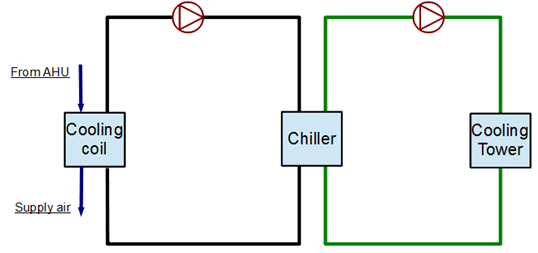
\includegraphics[width=0.9\textwidth, height=0.9\textheight, keepaspectratio=true]{media/image012.png}
\caption{Simple cooling system line diagram \protect \label{fig:simple-cooling-system-line-diagram}}
\end{figure}


\begin{figure}[hbtp] % fig 13
\centering
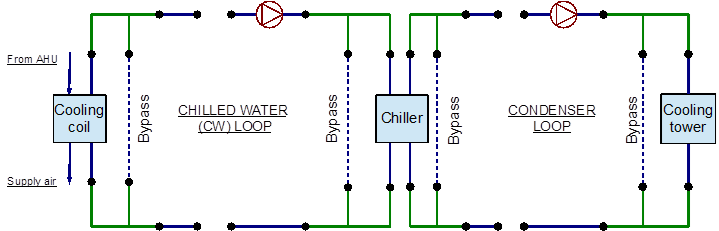
\includegraphics[width=0.9\textwidth, height=0.9\textheight, keepaspectratio=true]{media/image013.png}
\caption{EnergyPlus line diagram for the simple cooling system \protect \label{fig:energyplus-line-diagram}}
\end{figure}

The cooling system consists of a chilled water loop which is defined by the \emph{PlantLoop} object, and a condenser loop which is also defined by the \emph{PlantLoop} object. Identification of these loops in the system is critical for the process of modeling the system in the input file the flowchart for loop identification is provided in Figure~\ref{fig:flowchart-for-loop-identification}.

\begin{figure}[hbtp] % fig 14
\centering
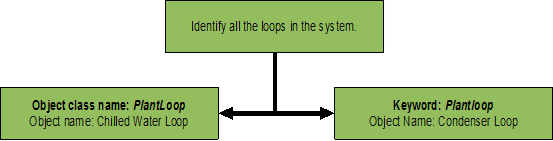
\includegraphics[width=0.9\textwidth, height=0.9\textheight, keepaspectratio=true]{media/image014.png}
\caption{Flowchart for loop identification \protect \label{fig:flowchart-for-loop-identification}}
\end{figure}
